\documentclass[12pt,hyperref,a4paper,UTF8]{ctexart}
\usepackage{HDUReport}
\usepackage{listings}
\usepackage{xcolor}
\usepackage{graphicx}
\usepackage{setspace}
\usepackage{float}
\setstretch{1.5} % 设置全局行距为1.5倍

\usepackage{enumitem} % 载入enumitem包以便自定义列表环境
\setlist[itemize]{itemsep=0pt, parsep=0pt} % 设置itemize环境的项目间距和段落间距

\setmainfont{Times New Roman} % 英文正文为Times New Roman


\usepackage{tikz}
\usetikzlibrary{shapes.geometric, arrows}
\usetikzlibrary{positioning, arrows.meta}
\usetikzlibrary{calc}
%封面页设置
{   
    %标题
    \title{ 
        \vspace{1cm}
        \heiti \Huge \textbf{《单片机原理及应用》作业报告} \par
        \vspace{1cm} 
        \heiti \Large {\underline{实验报告3第一部分:指定周期方波}   } 
        \vspace{3cm}
    
    }

    \author{
        \vspace{0.5cm}
        \kaishu\Large 学院\ \dlmu[9cm]{卓越学院} \\ %学院
        \vspace{0.5cm}
        \kaishu\Large 学号\ \dlmu[9cm]{23040447} \\ %班级
        \vspace{0.5cm}
        \kaishu\Large 姓名\ \dlmu[9cm]{陈文轩} \qquad  \\ %学号
        \vspace{0.5cm}
        \kaishu\Large 专业\ \dlmu[9cm]{智能硬件与系统(电子信息工程)} \qquad \\ %姓名 
    }
        
    \date{\today} % 默认为今天的日期,可以注释掉不显示日期
}
%%------------------------document环境开始------------------------%%
\begin{document}

%%-----------------------封面--------------------%%
\cover
\thispagestyle{empty} % 首页不显示页码
%%------------------摘要-------------%%
%\newpage
%\begin{abstract}




%\end{abstract}

%\thispagestyle{empty} % 首页不显示页码

%%--------------------------目录页------------------------%%
% \newpage
% \tableofcontents
% \thispagestyle{empty} % 目录不显示页码

%%------------------------正文页从这里开始-------------------%
\newpage
\setcounter{page}{1} % 让页码从正文开始编号

%%可选择这里也放一个标题
%\begin{center}
%    \title{ \Huge \textbf{{标题}}}
%\end{center}


\textbf{原题目:已知振荡频率为12MHz,用定时器/计数器T0,工作于方式1,实现从P1.0口输出周期为(20+学号后2位)ms的方波。分别用汇编语言和C语言,用中断方式和用查询方式编制程序。}

\section{第一部分:C语言查询方式输出方波}
\subsection{实验代码}

\begin{lstlisting}[language=C, caption={实验程序}]
/**
* @file square_wave.c
* @brief 使用51单片机定时器T0查询方式生成67ms方波(20ms+学号47)
* @details 
* - 晶振: 12MHz, 12T模式(1MHz机器周期)
* - 方波周期: 20ms + 学号后两位47ms = 67ms
* - 占空比: 50%(高低电平各33.5ms)
* - 输出引脚: P1.0
*/

#include <reg51.h>

/*============== 宏定义(参数集中管理,方便修改) ==============*/
#define FOSC        12000000UL  // 晶振频率12MHz(UL表示无符号长整型)
#define STUDENT_END 47          // 学号后两位数值(用于计算周期)
#define WAVE_MS     (20 + STUDENT_END)/2  // 半周期 = (20+47)/2 = 33.5ms
#define HALF_US     (WAVE_MS * 500)       // 半周期转微秒:33.5ms * 1000/2 = 33500μs
                                            // (500 = 1000μs/ms ÷ 2,因12T模式1μs/计数)
#define T0_LOAD     (65536 - HALF_US)     // 定时器初值 = 65536 - 33500 = 32036 (0x7D24)

/*============== 硬件接口定义 ==============*/
sbit WAVE_OUT = P1^0;  // 方波输出引脚(P1.0)

/*============== 主函数 ==============*/
void main() {
    /*----- 定时器T0初始化 -----*/
    TMOD = 0x01;       // 设置T0为模式1(16位定时器)
    TH0 = T0_LOAD / 256;  // 初值高字节 = 32036/256 = 0x7D
    TL0 = T0_LOAD % 256;  // 初值低字节 = 32036%256 = 0x24
    TR0 = 1;           // 启动定时器T0
    WAVE_OUT = 0;      // 初始输出低电平

    /*----- 主循环(查询方式生成方波) -----*/
    while(1) {
        while(!TF0);   // 阻塞等待定时器溢出(TF0=1时跳出)
        TF0 = 0;       // 必须手动清除溢出标志
        WAVE_OUT = ~WAVE_OUT;  // 电平翻转(33.5ms切换一次)
        
        /* 重装初值(保持周期精确) */
        TH0 = T0_LOAD / 256;  // 重新写入高字节
        TL0 = T0_LOAD % 256;  // 重新写入低字节
    }
}
   
    
\end{lstlisting}

\subsection{实验效果}

\begin{figure}[H] % [H] 表示强制当前位置插入
    \centering
    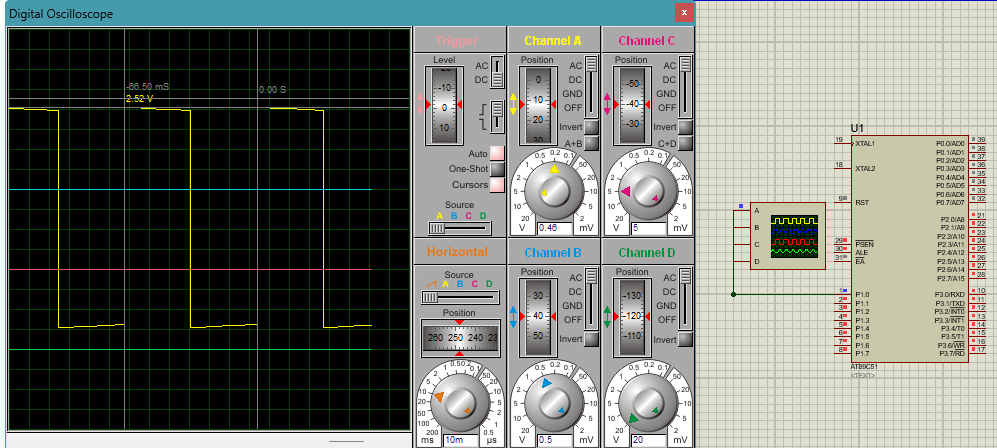
\includegraphics[width=1\textwidth]{figures/201.png} % 调整宽度为文本宽度的 80%
    \caption{Proteus示波器效果,周期手动测量约66.5ms,基本符合预期} % 图片标题
    \label{fig:example} % 图片标签,用于引用
\end{figure}






\subsection{流程图}

\begin{figure}[H]
    \centering
    \begin{tikzpicture}[
        node distance=1.5cm,
        startstop/.style={rectangle, rounded corners, minimum width=3cm, minimum height=1cm, text centered, draw=black, fill=red!30},
        process/.style={rectangle, minimum width=3cm, minimum height=1cm, text centered, draw=black, fill=blue!30},
        decision/.style={diamond, aspect=1.8, minimum width=2.5cm, minimum height=1.8cm, text centered, draw=black, fill=green!30},
        arrow/.style={thick, -Stealth}
    ]

        % ===== 主流程 =====
        \node (start) [startstop] {程序开始};
        \node (initLED) [process, below=of start] {初始化 LED};
        \node (initTimer) [process, below=of initLED] {初始化定时器};
        \node (loop) [process, below=of initTimer] {主循环等待中断};
        
        % ===== 中断处理 =====
        \node (interrupt) [decision, right=5cm of loop] {定时器中断触发?};
        \node (reload) [process, below=2cm of interrupt] {重装定时器初值};
        \node (countCheck) [decision, below=2cm of reload] {计数 $\geq$ 20?};
        \node (toggleLED) [process, left=3cm of countCheck] {LED 状态取反};
        \node (resetCount) [process, below=1cm of toggleLED] {计数器清零};

        % ===== 绝对坐标关键点定义 =====
        \coordinate (loopExit) at ($(loop.east)+(2cm,0)$);
        \coordinate (interruptReturn) at ($(interrupt.east)+(2cm,0)$);
        \coordinate (loopReturnTop) at ($(loop.north east)+(0,0.5cm)$);
        \coordinate (resetReturn) at ($(resetCount.west)-(2cm,0)$);

        % ===== 优化后的箭头路径 =====
        % 主流程
        \draw [arrow] (start) -- (initLED);
        \draw [arrow] (initLED) -- (initTimer);
        \draw [arrow] (initTimer) -- (loop);
        
        % 中断检测(完全重构路径)
        \draw [arrow] (loop.east) -- (loopExit) -- (interrupt.west);
        \draw [arrow] (interrupt.south) -- node[right] {是} (reload.north);
        
        % 中断"否"路径(关键优化)
        \draw [arrow] (interrupt.east) -- (interruptReturn) 
            -- ++(0,1.2cm) node[above left] {否} 
            -| (loopReturnTop) -- (loop.north east);
        
        % 中断处理
        \draw [arrow] (reload.south) -- (countCheck.north);
        \draw [arrow] (countCheck.west) -- node[above] {是} (toggleLED.east);
        \draw [arrow] (toggleLED.south) -- (resetCount.north);
        
        % 返回路径(双重避让)
        \draw [arrow] (resetCount.west) -- (resetReturn) 
            |- ($(loop.west)-(0,0.3cm)$) -- (loop.west);
        \draw [arrow] (countCheck.east) -- ++(1.5cm,0) node[above right] {否} 
            |- ($(reload.east)+(0,-0.5cm)$) -- (reload.east);

    \end{tikzpicture}
    \caption{单灯闪烁程序流程图}
    \label{fig:ultimate_flowchart}
\end{figure}


\section{第二部分:汇编语言中断方式输出方波}


\subsection{实验代码}

\begin{lstlisting}[language={[x86masm]Assembler}, caption={实验程序}]
; 宏/常量定义
CLK_FREQ    EQU 12000000   ; 12MHz
HALF_PERIOD EQU 16750      ; 半周期33.5ms (周期=20+47ms)
T0_RELOAD   EQU 65536-HALF_PERIOD  ; 计算初值
PORT_PIN    EQU P1.0       ; 输出引脚

ORG 0000H
LJMP MAIN
ORG 000BH
LJMP T0_ISR

ORG 0030H
MAIN:
    MOV TMOD, #01H        ; T0方式1
    MOV TH0, #(T0_RELOAD >> 8)   ; 高八位赋值
    MOV TL0, #(T0_RELOAD & 0FFH) ; 低八位赋值
    SETB ET0              ; 允许T0中断
    SETB EA               ; 开中断
    SETB TR0              ; 启动T0
    CLR PORT_PIN          ; 初始低电平
    SJMP $                ; 等待中断

T0_ISR:
    CPL PORT_PIN          ; 取反输出 半周期取反一次
    MOV TH0, #(T0_RELOAD >> 8)  ; 重装初值
    MOV TL0, #(T0_RELOAD & 0FFH)
    RETI
END
\end{lstlisting}

\subsection{实验效果}

\begin{figure}[H] % [H] 表示强制当前位置插入
    \centering
    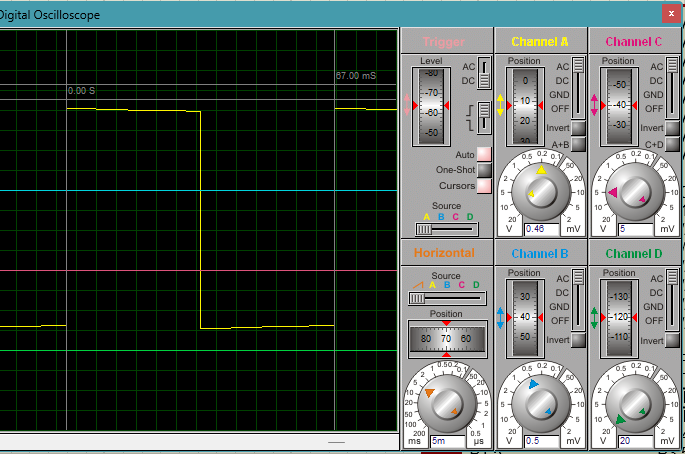
\includegraphics[width=1\textwidth]{figures/202.png} % 调整宽度为文本宽度的 80%
    \caption{Proteus示波器效果,周期手动测量为67ms} % 图片标题
    \label{fig:example} % 图片标签,用于引用
\end{figure}

\subsection{流程图}


\begin{figure}[H]
    \centering
    \begin{tikzpicture}[
        node distance=2cm,
        startstop/.style={rectangle, rounded corners, minimum width=3cm, minimum height=1cm, text centered, draw=black, fill=red!30},
        process/.style={rectangle, minimum width=3cm, minimum height=1cm, text centered, draw=black, fill=blue!30},
        decision/.style={diamond, aspect=1.8, minimum width=2.5cm, minimum height=1.8cm, text centered, draw=black, fill=green!30},
        arrow/.style={thick, -Stealth}
    ]

        % ===== 主流程 =====
        \node (start) [startstop] {程序开始};
        \node (initTimer) [process, below=of start] {初始化定时器T0};
        \node (initInterrupt) [process, below=of initTimer] {启用中断};
        \node (mainLoop) [process, below=of initInterrupt] {主循环等待中断};

        % ===== 中断处理 =====
        \node (interrupt) [decision, right=5cm of mainLoop] {中断触发?};
        \node (togglePin) [process, below=2cm of interrupt] {翻转输出引脚};
        \node (reloadTimer) [process, below=of togglePin] {重装定时器初值};

        % ===== 返回路径 =====
        \coordinate (returnPoint) at ($(mainLoop.east)+(2cm,0)$);
        \coordinate (noPath) at ($(interrupt.east)+(3cm,0)$);
        \coordinate (avoidOverlap) at ($(reloadTimer.west)+(-2cm,0)$);

        % ===== 箭头路径 =====
        % 主流程
        \draw [arrow] (start) -- (initTimer);
        \draw [arrow] (initTimer) -- (initInterrupt);
        \draw [arrow] (initInterrupt) -- (mainLoop);

        % 中断检测
        \draw [arrow] (mainLoop.east) -- (returnPoint) -- (interrupt.west);
        \draw [arrow] (interrupt.south) -- node[right] {是} (togglePin.north);
        \draw [arrow] (togglePin.south) -- (reloadTimer.north);

        % 返回主循环
        \draw [arrow] (reloadTimer.west) -- (avoidOverlap) |- ($(mainLoop.west)-(0,0.5cm)$) -- (mainLoop.west);

        % 中断“否”路径调整
        \draw [arrow] (interrupt.east) -- (noPath) node[above] {否} 
            |- ($(mainLoop.east)+(0,-1cm)$) -- (mainLoop.east);

    \end{tikzpicture}
    \caption{进一步优化后的汇编程序流程图}
    \label{fig:optimized_assembly_flowchart}
\end{figure}


\section{实验体会}

实验通过定时器模式1下,对于TL0,TX0定时器计数器的手动重装载,以及C语言与汇编语言的不同定时器溢出处理的实践(主线程查询与中断服务函数),
加深了我对定时器工作的理解,对于以后更加复杂的编程更有帮助。





\end{document}